Based on the presented idea, we design and present the prototype which consists of three components (see Figure \ref{fig:figure1}):
\begin{itemize}
\item 
\emph{The server} centrally manages all users information, bookings and machines status.

\item 
Each washing machine has a \emph{monitoring device} consisting of a RFID reader (for user authentication) and a screen which displays interactive instructions and information of the machine such as: machine id, remaining time of current job, current state of washing machine (\emph{AVAILABE} - there is still enough time before the next reservation begins, \emph{USED IN A MOMENT} - next reservation will begin shortly, \emph{RESERVED} - the machine was already booked at that moment, \emph{IN USE} - machine is running, \emph{FINISHED} - washing has just finished), etc.

\item 
\emph{{\toolname}} is an Android application which allows users to reserve and manage bookings, observe the current states of the machines. The application also uses in-app notification, SMS message and email to remind users for upcoming bookings or finished jobs. There are two bar charts displayed in the application which illustrates the numbers of bookings in previous week by hours and by days. Users could use these statistics to plan their ``laundry strategy'' of the week.

The \emph{Home} interface (see Figure \ref {fig:home}) displays all information about the user. This is where gamification idea is implemented. In this tab, users could find their avatars, names, balance and points, levels and progression as well as messages about their activities. There are also buttons allowing them to access leader board (see Figure \ref{fig:leaderboard}), report a person or add money to their accounts. 

\end{itemize}
\begin{figure}[h]
\centering
  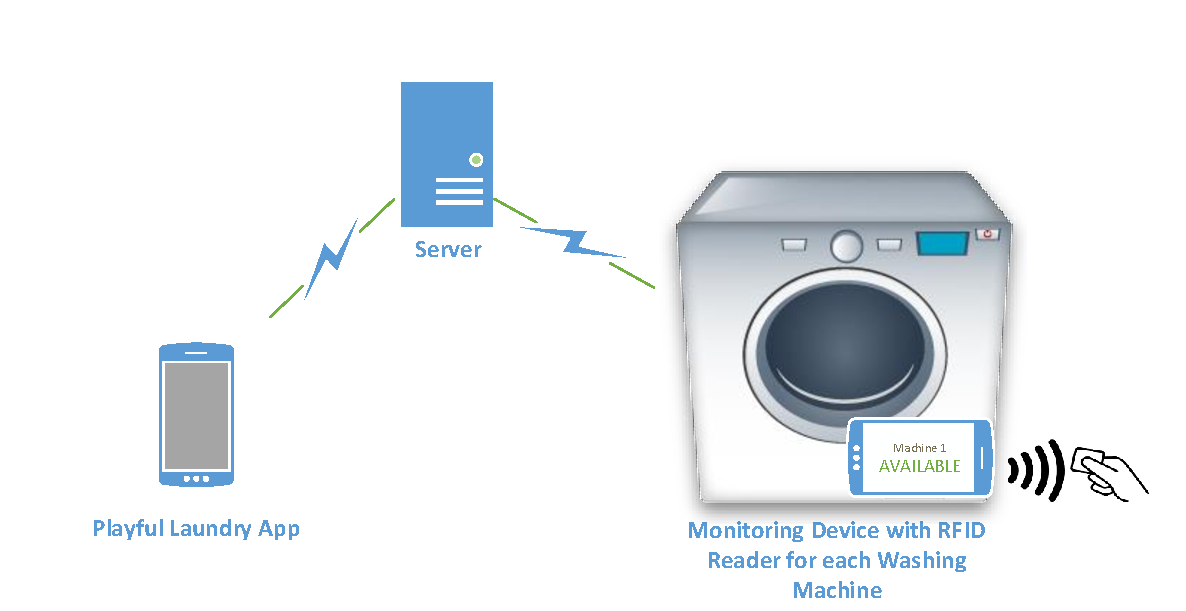
\includegraphics[width=.8\columnwidth]{figures/overview}
  \caption{Three components of the booking system.}~\label{fig:figure1}
\end{figure}

\begin{figure}[h]%
    \centering
   \subfloat[Home]{{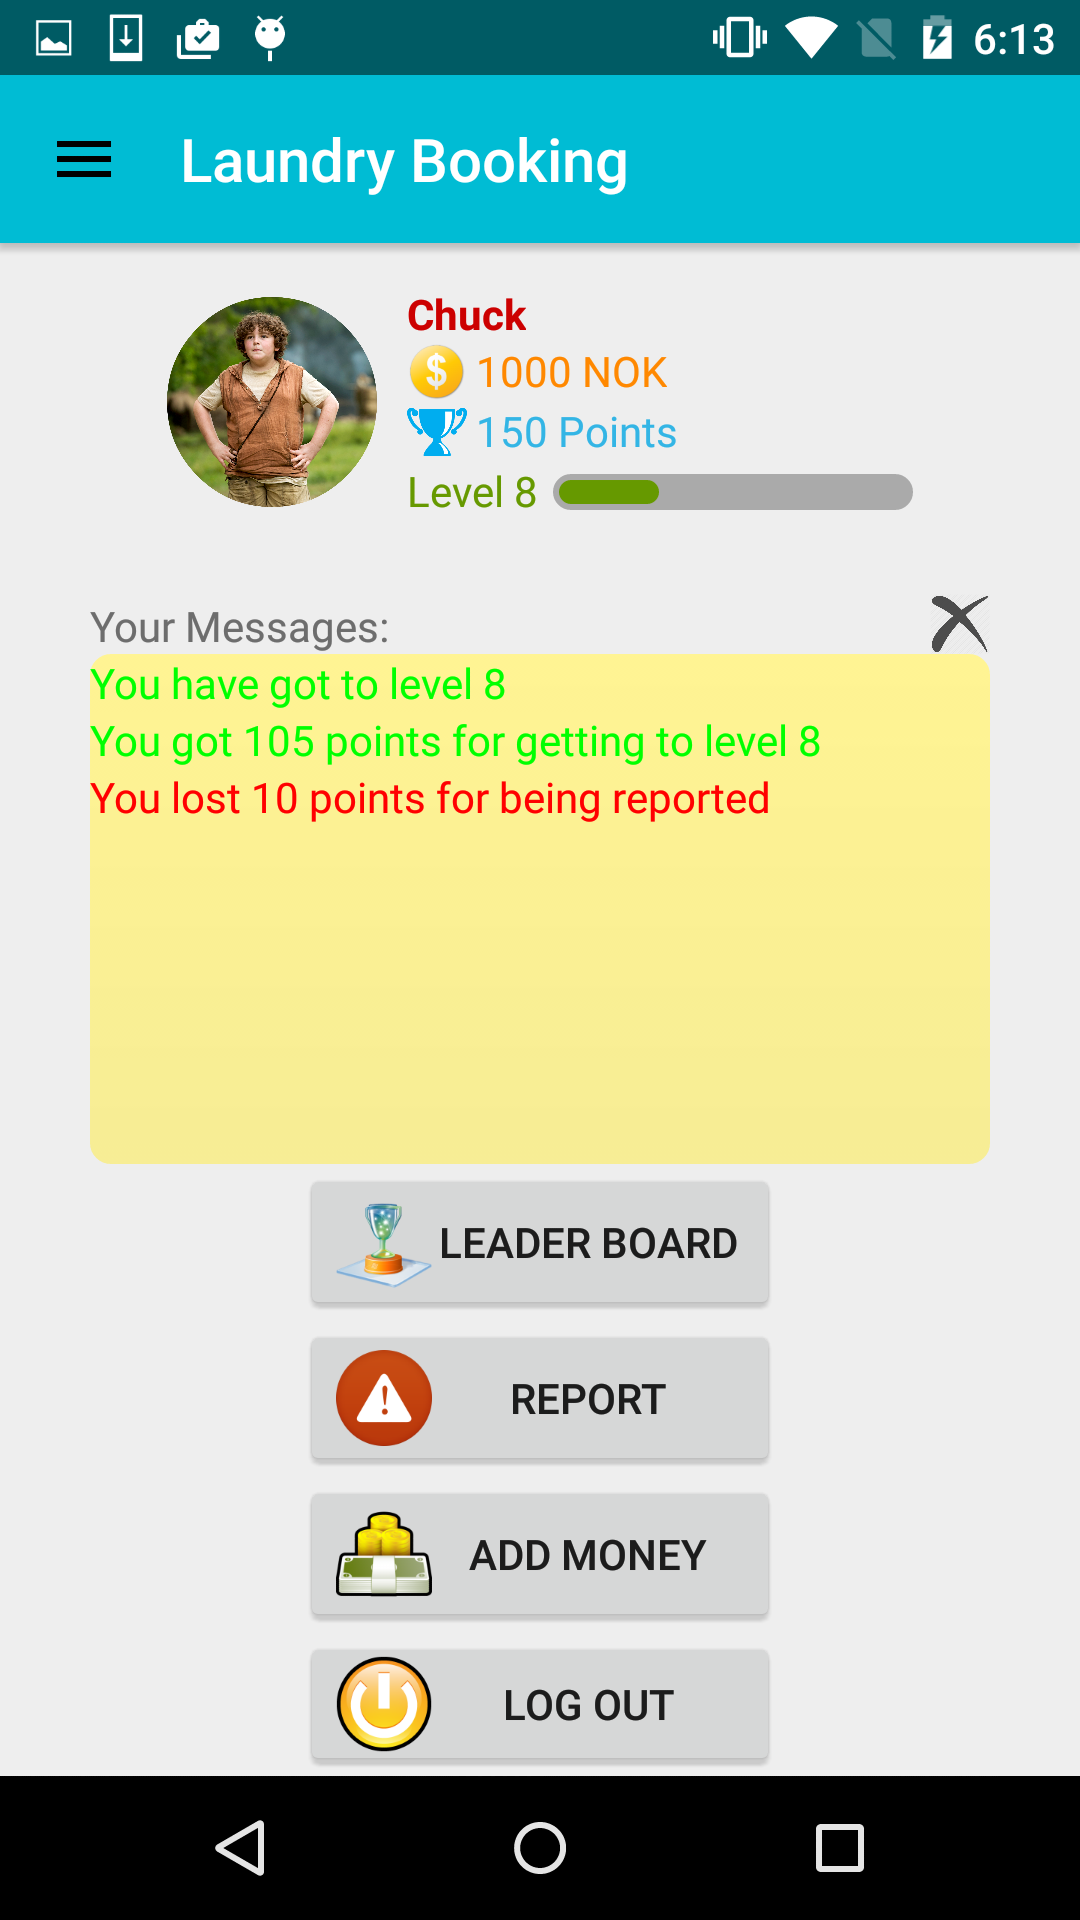
\includegraphics[width=0.4\columnwidth]{figures/home} \label{fig:home} }}
    %\qquad
    \subfloat[Leader Board]{{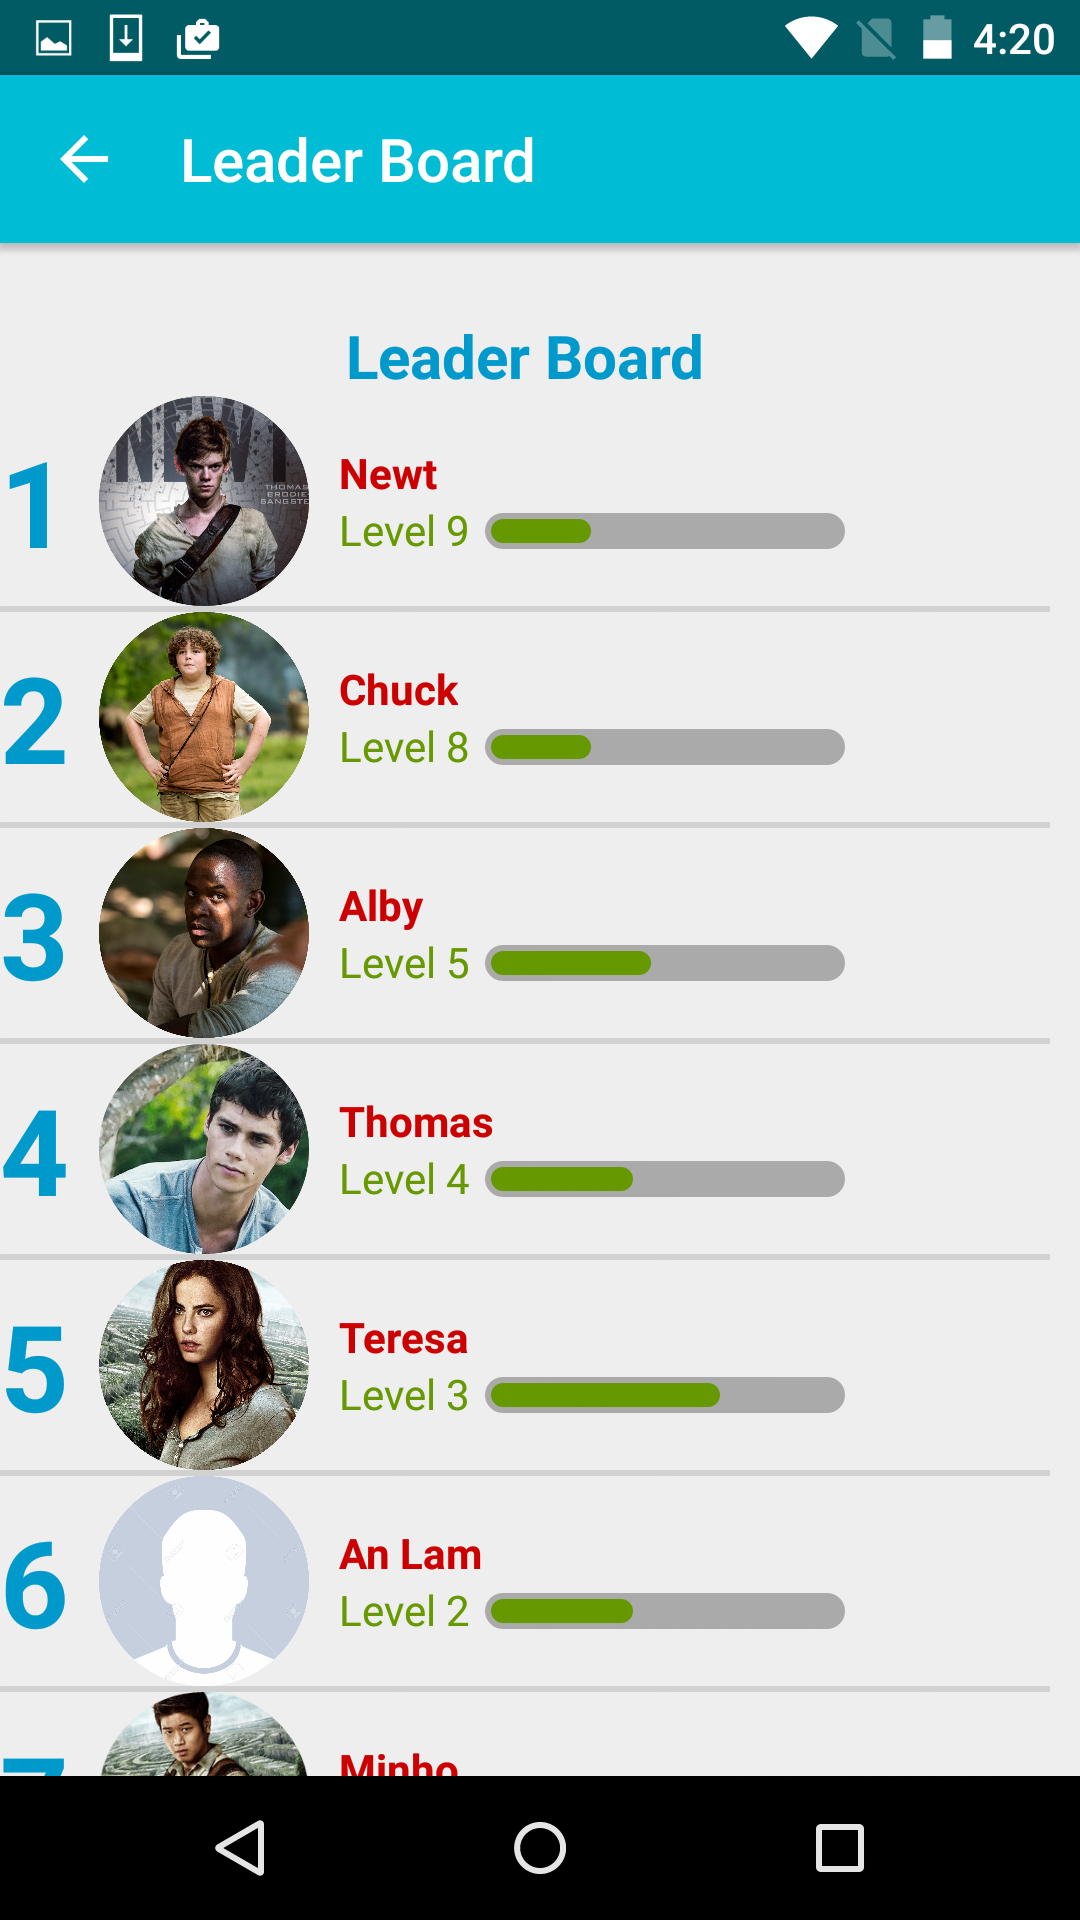
\includegraphics[width=0.4\columnwidth]{figures/leaderboard} \label{fig:leaderboard} }}
		\caption{Home Page and Leader board.}%
    \label{fig:figure5}
\end{figure}